\documentclass[a4paper,12pt]{article}
\usepackage[utf8]{inputenc}
\usepackage{natbib}
\usepackage{graphicx}


\title{\vspace{4cm} Embedded Hardware Design \\ Project Report \\ \\\begin{flushright} \small{- Group 8} \end{flushright}\hline}
\date{}

\begin{document}

\begin{titlepage}
    
    \maketitle
    
    \vspace{5cm}
    \textbf{Team members:}
        \begin{table}[h!]
            \begin{tabular}{c c}
         Vishal Goyal & 201501421 \\
         Chahak Mehta & 201501422\\
         Swastika Nayak & 201501423\\
         Ayub Subhaniya & 201501433\\
         Siddhraj Sisodiya & 201501434
            \end{tabular}
        \end{table}
\end{titlepage}

\section{Project Details}

\subsection{Topic}

\quad Raspberry Pi powered, voice controlled $Chess-bot^{{\scriptsize{\cite{link}$
}}

\textbf{Team leader:} Chahak Mehta (201501422)

\subsection{Project goal and deliverables}

	A self-analyzing chess-bot, inspired from the magical chess from the book \textit{Harry Potter and The Sorcerer's Stone} against which a player can play by giving the voice commands.\\\\
	Also works as a fan-favourite collectible which can be further commercialized as a Harry Potter themed chess-board.

\subsection{Equipment required}

\begin{itemize}

    \item Raspberry PI 3
    \item USB microphone
    \item ULN2003 5 Line 4 Phase
    \item Large Chess Board with pieces
    \item 1 10k 1/4 Watt resistors
    \item 30AWG Wire
    \item Magnets to fit pieces
    \item 1 Large Neodymium Magnet
    \item 2 Pairs of 24'' Drawer Bearings 
    \item 2 Stepper Motors (28BYJ-48)
    \item 2 Vex Rack and Gear Sets 
    \item 1 Standard Hobby Servo
    \item 1 2'x2'x1/2'' MDF board
    \item scrap wood 1''x2''

\end{itemize} 

\subsection{Working}

\subsubsection{Circuit Diagram}

\begin{figure}[h!]
    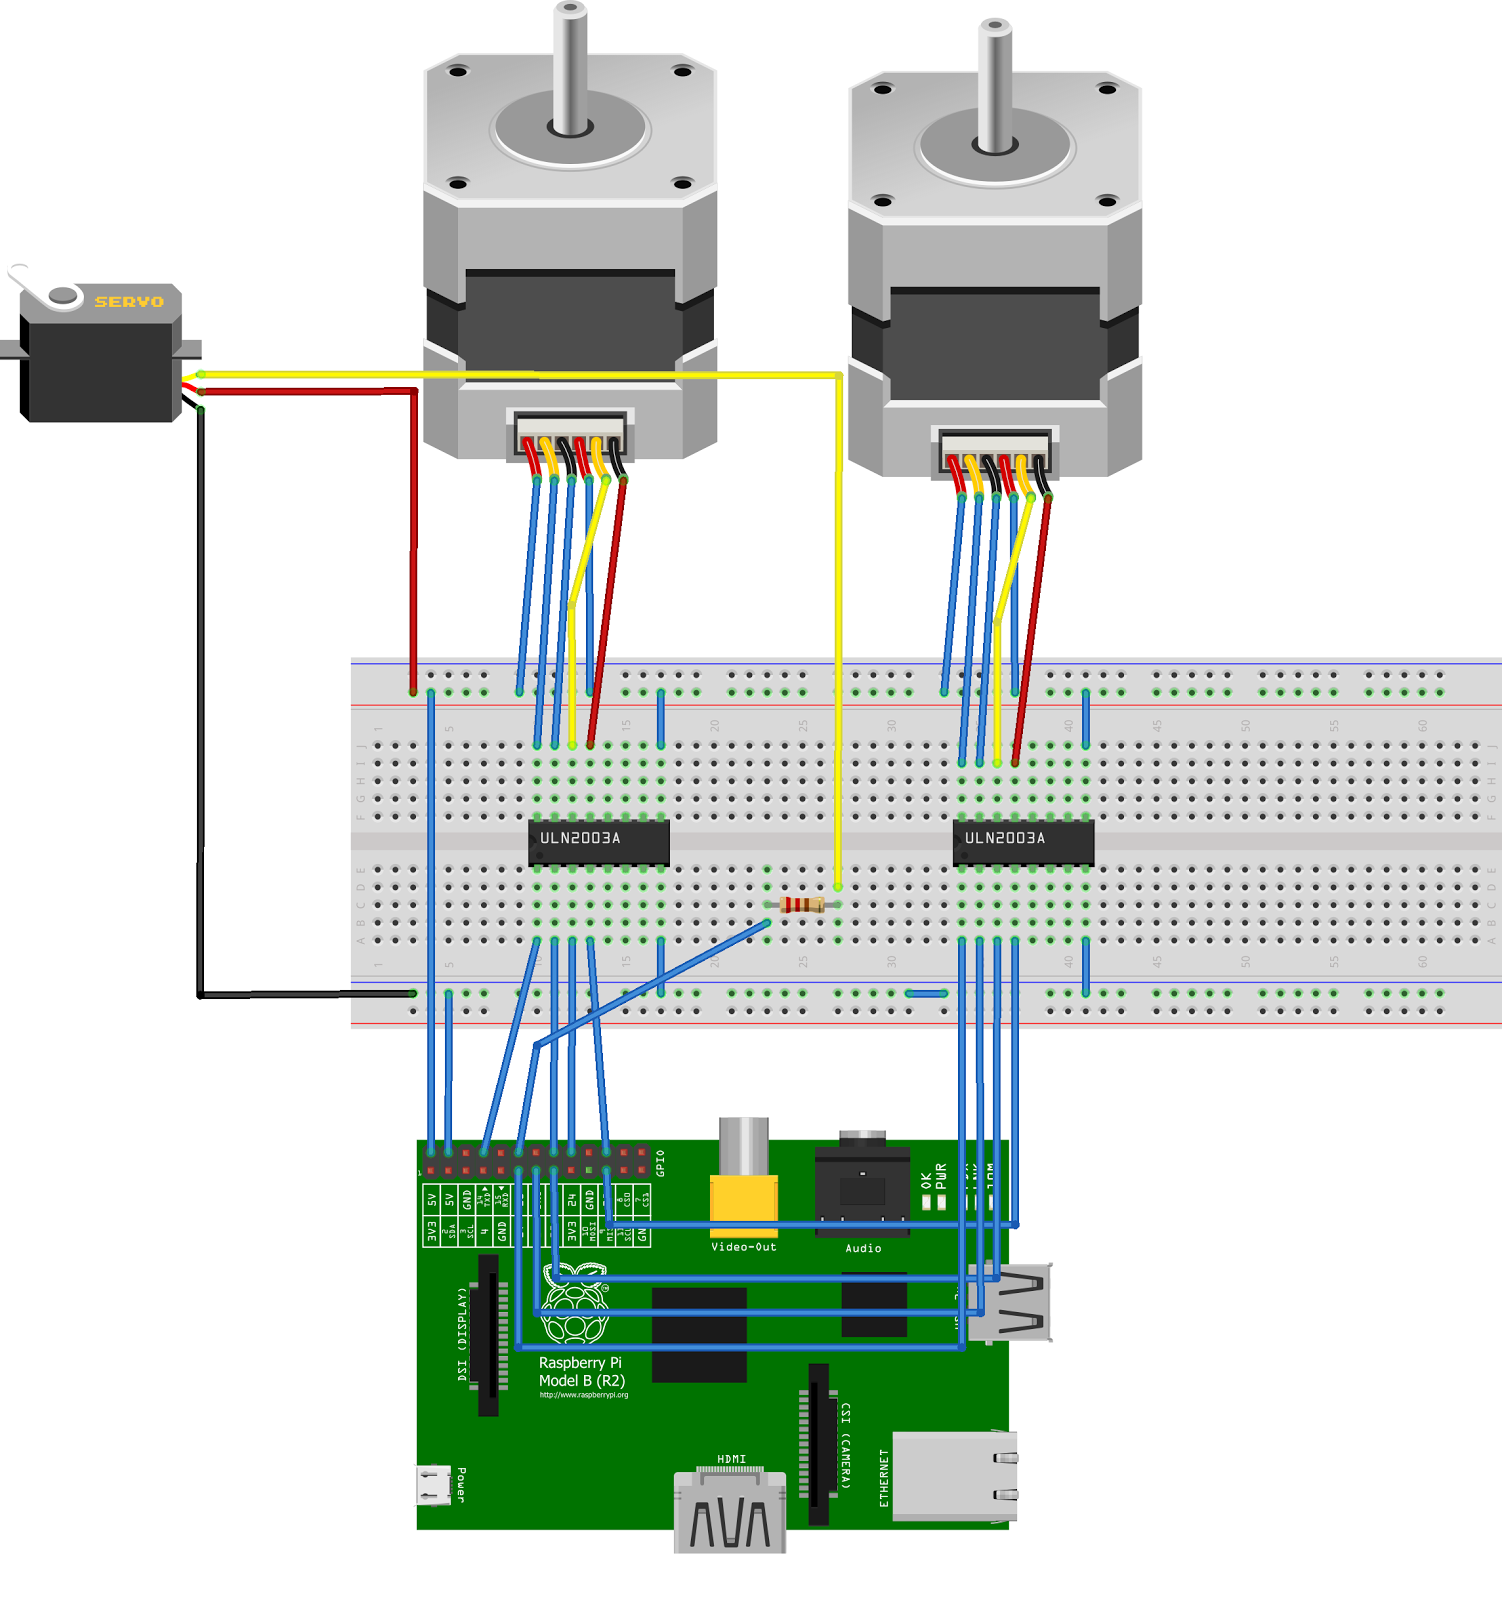
\includegraphics[scale = 0.2]{Circuit_Diagram_Chess.png}
    \caption{Circuit diagram showing hardware connections}
    \label{fig:ckt_dig}
\end{figure}

	The Figure \ref{fig:ckt_dig} shows 2 stepper motors and a servo controlled by a Raspberry Pi. The stepper motors are connected with drive test module boards which are connected with raspberry pi. These motors are connected under the chess-board as shown in \textit{Figure \ref{fig:motors}} in the next section.

\newpage
\subsubsection{Additional working details}
\begin{figure}[h!]
    \centering
    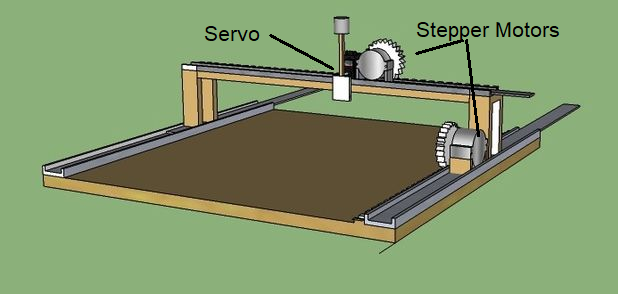
\includegraphics[scale = 0.7]{Chess_Hand.png}
    \caption{Stacking of motors under the chess board}
    \label{fig:motors}
\end{figure}

    The two stepper motors and a servo motor are connected under under the chess-board as shown in \textit{Figure \ref{fig:motors}}.\\
    \quad One of the stepper motors is placed horizontally and the other is placed vertically. These stepper motors control the motion of the pieces in X and Y directions respectively. Furthermore, the servo motor, stacked on the horizontal stepper motor acts as a magnetic hand which is then used to move the piece to the destination using the stepper motors.

\subsection{Work distribution}

\begin{itemize}
    \item Coding: Ayub, Siddhraj, Vishal
    \item Hardware implementation: Swastika, Chahak
    \item Documentation: Chahak
\end{itemize}


\bibliographystyle{plain}
\bibliography{references}

\end{document}
